\chapter{Panel Data Methods}
	\begin{definition}[Panel data]
		Panel data is cross-sectional data, observed over time for each individual.
	\end{definition}
	An example of such data is the multivariate linear regression model given by
	\begin{align}
		y_{it} = \beta_0 +\beta_1 x_{1,it}+\dots +\beta_k x_{k,it}+u_{it}
	\end{align}
	where $i=1,2,\dots,n$ indexes individuals, while $t=1,2\dots,T$ simultaneously indexes the observation time for individual $i$.
	
	Another seemingly similar type of data is called \textit{repeated cross section}; note this is not the same a panel data, as it does not necessarily hold that the same individuals are observed over time.
	
	For panel data, in general we can decompose the error term $u_i$ into a time-invariant component $a_i$ and a de-trended error, $v_{it}$,
	\begin{align}
		y_{it} = \beta_0 +\beta_1 x_{1,it}+ \cdots +\beta_k x_{k,it} +a_i +v_{it}
	\end{align}
	$a_i$ represents the `effect of being individual $i$'. A big problem for us econometricians is that $a_i$ can be highly correlated with our regressors, and hence induce bias. Although this problem is not unique to panel data, the nature/strength of panel data allows us to overcome this issue. We will two major estimators:
	\begin{enumerate}
		\item \textbf{First Differences (FD)}
		\item \textbf{Fixed Effects (FE)}
	\end{enumerate}
	In this chapter we will also discuss the Difference-in-Differences (DiD) estimator, a method to deal with before and after treatment data with two groups - a specific kind of panel data.
	
    \section{First Differences (FD)}
        \subsection{Estimator derivation}
            Define $\Delta y_{it} = y_{it} - y_{i(t-1)}$ as the change in the outcome variable over time for individual $i$.
            \begin{definition}[First differences estimator]
                Assuming the linear regression model, the \textit{First Differences} (FD) estimator, is the OLS estimator of the regression model (without constant):
    			\begin{align}
    				\Delta y_{it} = \beta_1 \Delta x_{1,it} + \dots +\beta_k \Delta x_{k,it} + \Delta v_{it}
    			\end{align}
    			where $\Delta x_{j,it} = x_{j,it} - x_{j,i(t-1)}$.
    		\end{definition}
    		\begin{proof}
    			Assuming the linear regression model, we have
    			\begin{align*}
    				\Delta y_{it}
    		      		&:=  y_{it} - y_{i,t-1}\\
    					&= \left(\beta_0 +\beta_1 x_{1,it}+\cdots+\beta_k x_{k,it} +a_i +v_{it}\right) \\
    					&\phantom{-}\qquad- \left(\beta_0 +\beta_1 x_{1,i(t-1)}+ \cdots +\beta_k x_{k,i(t-1)} +a_i +v_{i(t-1)}\right)\\
    					&= 
    					(\beta_0-\beta_0 ) + (\beta_1x_{1,it}-\beta_1x_{1,i(t-1)} ) +\\
    					&\phantom{=}\qquad\dots+ (\beta_k x_{k,it}-\beta_k x_{k,i(t-1)} ) +(a_i-a_i)+(v_{it}-v_{i(t-1)}) \\
    					&= \beta_1 \Delta x_{1,it} + \dots +\beta_k \Delta x_{k,it} + \Delta v_{it}
                \end{align*}
            \end{proof}
            
            Note the individual level effect is differenced out, as well as the intercept. Also note we lose the first observation for each $i$. Also note any variable which are time invariant, i.e. don’t change over time, are also differenced out, e.g. blood type.
            
		\subsection{Implementation}
			To summarise the previous section, we first
			\begin{enumerate}[(1)]
				\item calculate the first difference, that is $\{\Delta y_{it}, \Delta x_{1,it} ,\dots ,\Delta x_{k,it}\}$
				\item estimate via OLS with no constant
			\end{enumerate}
			To implement this in STATA, refer to Listing \ref{lst:panel/FD/implement}
			\begin{sexylisting}[colback=white, label=lst:panel/FD/implement]{First Differences Estimator}
//	(setup) Tell STATA we have panel data
	xtset id time

//	(setup) Sort the data by id and time
	sort id time

//	(1) Create differences variables
	gen diff_y = d.y
	gen diff_x_1 = d.x_1
	gen diff_x_2 = d.x_2

//	(2) Run the regression with no constant (nocons)
	reg diff_y diff_x_1 diff_x_2, robust nocons
			\end{sexylisting}
			
		\section{Fixed Effects (FE)}
			\subsection{Estimator derivation}
				To derive the FE estimator, we first demean the data across time, for each individual. Let $\tilde y_{it} := y_{it} - \bar y_{i}, \tilde x_{j,it} = x_{j,it}-\bar x_{j,i}$ and $\tilde v_{it} = v_{it}-\bar v_i$. Any variable that doesn’t change over time becomes 0 after being demeaned, for example $\tilde a_i = 0$, and so we cannot estimate their effect. 
				
				\begin{definition}
					The \textit{fixed effects }estimator is defined the OLS estimator of the regression model
					\begin{align}
						\tilde y_{it} = \beta_1\tilde x_{1,it}+\dots \beta_k\tilde x_{k,it} + \tilde u_{it}
					\end{align}
				\end{definition}
				This method is quite \textit{tedious} so thankfully there is an alternative method, involving dummy variables.
				
			\subsection{Dummy variable implementation}
				Rather than demean every variable, we can instead introduce a dummy variable for all but one of the individuals (to avoid dummy variable trap). Therefore we estimate
				\begin{align}
					\textstyle y_{it} = \beta_0 +\beta_1 x_{1,it}+\dots +\beta_k x_{k,it} +\sum_{i=1}^{n-1}a_i\delta_i +v_{it}
				\end{align}
				
				\noindent\textbf{Interpretation.} How can we interpret the value of $a_i$? It is the average difference in $y_i$ for being associated with individual $i$, compared to the excluded individual, called the `fixed effect'.
				
				In STATA, we implement this as in Listing \ref{lst:panel/FE/dummy}
				\begin{sexylisting}[colback=white, label=lst:panel/FE/dummy]{Fixed Effects Estimator}
//	(setup) Tell STATA we have panel data
	xtset id time

//	(setup) Sort the data by id and time
	sort id time

//	There are two ways to run the regression.
//	xtreg is more elegant, 
//	but we present the other way for completeness.

//	Option 1: Run the regression with xtreg and fe
	xtreg y x_1 x_2 , fe

//	Option 2: Run the regression normally
	xi: reg y x_1 x_2  i.id,
				\end{sexylisting}
				
			\subsection{Time fixed effects}
				We can extend the individual fixed effect to time fixed effects, i.e. the effect of being in a particular time period. We can interpret time and individual fixed effects
				\begin{align}
					\textstyle y_{it} = \beta_0 + \sum_{j=1}^k \beta_j x_{j,it}+\sum_{i=1}^{n-1}a_i\delta_i +\sum_{t=1}^{T-1}c_t\gamma_t+v_{it}
				\end{align}
				where $c_t$ is the effect of being in period $t$, and $\gamma$ is the dummy for time $t$.
				
				In STATA this is peformed as in Listing \ref{lst:panel/FE/dummy_time}
				\begin{sexylisting}[colback=white, label=lst:panel/FE/dummy_time]{FE estimator with time fixed effects}
//	(setup) Tell STATA we have panel data 
	xtset id time

//	(setup) Sort the data by id and time
	sort id time

//	Option 1: Run the regression with xtreg and fe
	xtreg y x_1 x_2 i.time, fe

//	Option 2: Run the regression normally
	xi: reg y x_1 x_2 i.id i.time,
				\end{sexylisting}
				
		\section{Comparison of FE and FD}
			Fixed effects estimation allows us to measure the `fixed effects' and compare them, whereas first differences already difference them out. It turns out that fixed effects is more commonly used due to `simplicity' to implement and the benefits of estimating `fixed effects'. Some additional facts to note that are not examined are:
			\begin{itemize}
				\item The estimators are identical if $T=2$.
				\item FD has smaller variance if the error is a random walk, $u_it = u_{i(t-1)} + \varepsilon_{it}$, but larger if $u_{it}$ is independent.
				\item FD requires weaker technical assumptions for consistency: $\forall j\leq k,t\leq T,  \ \cov{\Delta u_{it},\Delta x_{j,it}} = 0$ and for FE: $\forall j\leq k,t\leq T,s\leq T,  \ \cov{\Delta u_{is},\Delta x_{j,it}}=0$
			\end{itemize}
			In summary, with panel data \textbf{the default strategy should be to estimate a fixed effects model and include time fixed effects}. However, depending on the conditions of the error term, the first difference estimator can be superior especially if the number of time periods is small.
			
    \section{Difference-in-Differences (DiD)}
        The ideal method to estimate a treatment effect is in a randomised trial. Economists rarely have the luxury of running experiments, and we must make use of observational data to estimate treatment effects. Difference-in-differences is a common attempt to create unbiased estimates.
        
        We first set up the model in which DiD is applied. Consistent with notation throughout the book, let $D_{it}$ be a dummy variable denoting treatment. In addition, we assume we have two time periods, $t= 0,1$, where $t=0$ corresponds to pre-treatment, and $t=1$ is post-treatment. Note this is without loss of generality as we can define $t$ as an indicator/dummy variable of $s$ which records the actual time; for instance $t = \ind_{s\geq\theta}$ if treatment occurs in period $\theta$. Let $T,C$ be the set of individuals in treated and control groups respectively.


        \subsection{Estimator derivation}
            Suppose we have the model
			\begin{align}
				y_{it} = \delta D_{it} + \gamma_i + \lambda_t + v_{it}
			\end{align}
			where $\delta$ is the effect of treatment, $\gamma_i$ controls for the group (treatment/control) taking values $\gamma_C,\gamma_T$  and $\lambda_t$ controls for the time period (pre/post). The dummy is slightly modified and takes the form
			\begin{align}
				D_{it} =
				\begin{cases}
					1 & \text{if }i\in T\text{ and } t=1\\
					0 & \text{otherwise}
				\end{cases}
			\end{align}

            \begin{definition}[DiD estimator]
                The \textit{Difference-in-Differences} (DiD) estimator is defined as
                \begin{align}
                    \hat\delta_\text{DiD}
                        &= \left(\bar y_\text{post}^\text{treat}-\bar y_\text{pre}^\text{treat}\right)-\left(\bar y_\text{post}^\text{control}-\bar y_\text{post}^\text{control}\right)\\
                        &=\sum_{i\in T} (y_{i1} - y_{i0}) - \sum_{i\in C} (y_{i1} - y_{i0})
                \end{align}
                It is called difference-in-difference as we take the difference in outcomes over time, then difference the change in outcome between the two groups.
            \end{definition}
            \begin{proof}
                For
                \begin{itemize}
                    \item \textbf{control group, $i\in C$}
                    \begin{align}
                        & y_{i0} = \gamma_C + \lambda_0 + v_{i0}   \\
                        & y_{i1} = \gamma_C + \lambda_1 + v_{i1}   
                    \end{align}
                    \item \textbf{treatment group, $i\in T$}
                    \begin{align}
                        & y_{i0} = \gamma_T + \lambda_0 + v_{i0}   \\
                        & y_{i1} = \delta + \gamma_T + \lambda_1 + v_{i1}   
                    \end{align}
                \end{itemize}
                We would like to know $\delta$. Consider
                \begin{align}
                    (y_{i1} - y_{i0})\ind_{i\in T} - (y_{i1} - y_{i0})\ind_{i\in C}
                        &= \left[(\delta + \gamma_T + \lambda_1 + v_{i1})- (\gamma_T + \lambda_0 + v_{i0})\right]\ind_{i\in T}\nonumber\\
                        &\phantom{=}\qquad  - \left[(\gamma_C + \lambda_1 + v_{i1}) - (\gamma_C + \lambda_0 + v_{i0})\right]\ind_{i\in C}     \\
                        &= \delta + (v_{i1} - v_{i0})\ind_{i\in T} - (v_{i1} - v_{i0})\ind_{i\in C}
                \end{align}
                Taking expectations yields
                \begin{align}
                    \expect{(y_{i1} - y_{i0})\ind_{i\in T} - (y_{i1} - y_{i0})\ind_{i\in C}} = \delta
                \end{align}
                The DiD estimator is therefore the MM estimator of the above expression.
            \end{proof}

        \subsection{Regression representation}
            We can represent the above in a regression with dummy variables as follows. Keeping the same notation, we have
            \begin{align}
                y_{it} = \beta_0 +\beta_1 t + \beta_2 \ind_{i\in T} + \beta_{3}(t\cdot \ind_{i\in T}) + v_{it}
            \end{align}
            where $\beta_1$ is the difference in being in period post vs pre, $\beta_2$ is the difference just for being in the treated group, and $\beta_3$ is the identified treatment effect.

        \subsection{Implementation}
            To implement DiD in STATA refer to Listing \ref{lst:panel/DiD/implement}.
            \begin{sexylisting}[colback=white, label=lst:panel/DiD/implement]{DiD estimator}
//  Split the data into pre and post (year is the cutoff)
    gen post = time >= year

//  Define the treated dummy and the interaction term
    gen treat = id == treated
    gen treat_post = post * treat

//  Run the DiD regression
    reg y treat post treat_post, robust
            \end{sexylisting}

        \subsection{Parallel trends}
            The important assumption underlying DiD is called ‘parallel trends’ or the effect of time, i.e. $\lambda_1 - \lambda_0$ is equal in both treated and control groups.

            In Figure \ref{fig:panel/DiD/parallel_trend}, we can see that the assumption of parallel trends in the regression representation means that $\beta_1$ lifts both the red and green line. If parallel trends was not true and there was no time effect on the treated group, dotted/red line would be flat.

            \begin{figure}
                \centering
                

\tikzset{every picture/.style={line width=0.75pt}} %set default line width to 0.75pt        

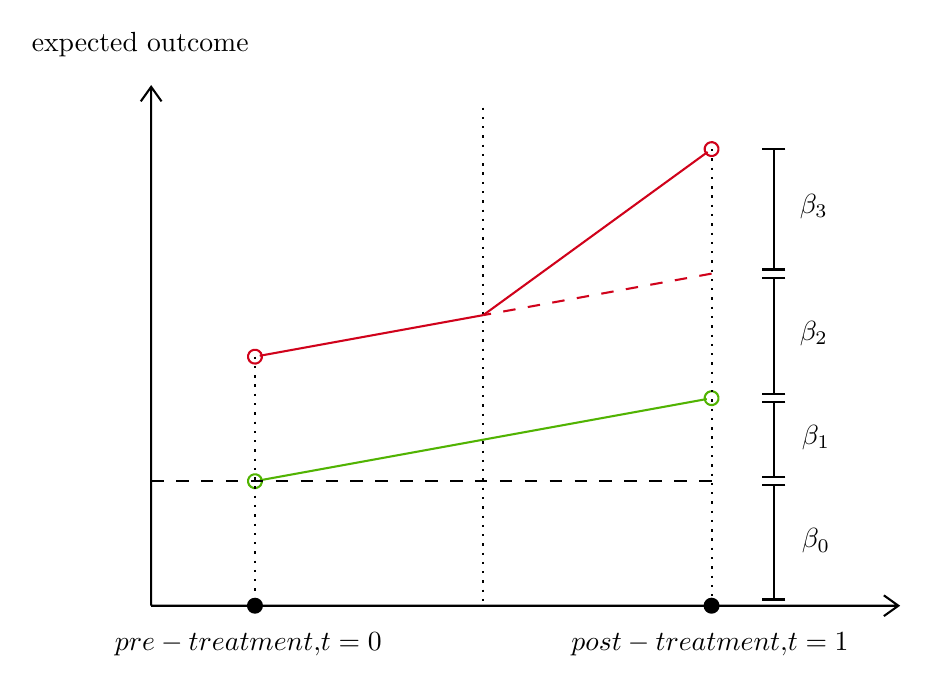
\begin{tikzpicture}[x=0.75pt,y=0.75pt,yscale=-1,xscale=1]
%uncomment if require: \path (0,466); %set diagram left start at 0, and has height of 466

%Shape: Axis 2D [id:dp8173979251061212] 
\draw  (200,320) -- (560,320)(200,70) -- (200,320) -- cycle (553,315) -- (560,320) -- (553,325) (195,77) -- (200,70) -- (205,77)  ;
%Straight Lines [id:da6661208351165583] 
\draw  [dash pattern={on 0.84pt off 2.51pt}]  (360,80) -- (360,320) ;
%Straight Lines [id:da9496708268405148] 
\draw [color={rgb, 255:red, 81; green, 179; blue, 2 }  ,draw opacity=1 ]   (252.31,259.58) -- (467.69,220.42) ;
\draw [shift={(470,220)}, rotate = 349.7] [color={rgb, 255:red, 81; green, 179; blue, 2 }  ,draw opacity=1 ][line width=0.75]      (0, 0) circle [x radius= 3.35, y radius= 3.35]   ;
\draw [shift={(250,260)}, rotate = 349.7] [color={rgb, 255:red, 81; green, 179; blue, 2 }  ,draw opacity=1 ][line width=0.75]      (0, 0) circle [x radius= 3.35, y radius= 3.35]   ;
%Straight Lines [id:da7605028786786207] 
\draw [color={rgb, 255:red, 208; green, 2; blue, 27 }  ,draw opacity=1 ]   (252.31,199.58) -- (360,180) ;
\draw [shift={(250,200)}, rotate = 349.7] [color={rgb, 255:red, 208; green, 2; blue, 27 }  ,draw opacity=1 ][line width=0.75]      (0, 0) circle [x radius= 3.35, y radius= 3.35]   ;
%Straight Lines [id:da6204156956628457] 
\draw [color={rgb, 255:red, 208; green, 2; blue, 27 }  ,draw opacity=1 ]   (468.1,101.38) -- (360,180) ;
\draw [shift={(470,100)}, rotate = 143.97] [color={rgb, 255:red, 208; green, 2; blue, 27 }  ,draw opacity=1 ][line width=0.75]      (0, 0) circle [x radius= 3.35, y radius= 3.35]   ;
%Straight Lines [id:da7633688703424713] 
\draw [color={rgb, 255:red, 208; green, 2; blue, 27 }  ,draw opacity=1 ] [dash pattern={on 4.5pt off 4.5pt}]  (470,160) -- (360,180) ;
%Straight Lines [id:da8118050967929765] 
\draw  [dash pattern={on 4.5pt off 4.5pt}]  (200,260) -- (470,260) ;
%Straight Lines [id:da5126836868598805] 
\draw    (500,262) -- (500,317) ;
\draw [shift={(500,317)}, rotate = 270] [color={rgb, 255:red, 0; green, 0; blue, 0 }  ][line width=0.75]    (0,5.59) -- (0,-5.59)   ;
\draw [shift={(500,262)}, rotate = 270] [color={rgb, 255:red, 0; green, 0; blue, 0 }  ][line width=0.75]    (0,5.59) -- (0,-5.59)   ;

%Straight Lines [id:da3500991397548453] 
\draw    (500,222) -- (500,258) ;
\draw [shift={(500,258)}, rotate = 270] [color={rgb, 255:red, 0; green, 0; blue, 0 }  ][line width=0.75]    (0,5.59) -- (0,-5.59)   ;
\draw [shift={(500,222)}, rotate = 270] [color={rgb, 255:red, 0; green, 0; blue, 0 }  ][line width=0.75]    (0,5.59) -- (0,-5.59)   ;

%Straight Lines [id:da4371401624287816] 
\draw    (500,162) -- (500,218) ;
\draw [shift={(500,218)}, rotate = 270] [color={rgb, 255:red, 0; green, 0; blue, 0 }  ][line width=0.75]    (0,5.59) -- (0,-5.59)   ;
\draw [shift={(500,162)}, rotate = 270] [color={rgb, 255:red, 0; green, 0; blue, 0 }  ][line width=0.75]    (0,5.59) -- (0,-5.59)   ;

%Straight Lines [id:da35598018492557226] 
\draw    (500,100) -- (500,158) ;
\draw [shift={(500,158)}, rotate = 270] [color={rgb, 255:red, 0; green, 0; blue, 0 }  ][line width=0.75]    (0,5.59) -- (0,-5.59)   ;
\draw [shift={(500,100)}, rotate = 270] [color={rgb, 255:red, 0; green, 0; blue, 0 }  ][line width=0.75]    (0,5.59) -- (0,-5.59)   ;

%Straight Lines [id:da32753381874785703] 
\draw  [dash pattern={on 0.84pt off 2.51pt}]  (470,100) -- (470,320) ;
\draw [shift={(470,320)}, rotate = 90] [color={rgb, 255:red, 0; green, 0; blue, 0 }  ][fill={rgb, 255:red, 0; green, 0; blue, 0 }  ][line width=0.75]      (0, 0) circle [x radius= 3.35, y radius= 3.35]   ;
%Straight Lines [id:da9408422259752088] 
\draw  [dash pattern={on 0.84pt off 2.51pt}]  (250,200) -- (250,320) ;
\draw [shift={(250,320)}, rotate = 90] [color={rgb, 255:red, 0; green, 0; blue, 0 }  ][fill={rgb, 255:red, 0; green, 0; blue, 0 }  ][line width=0.75]      (0, 0) circle [x radius= 3.35, y radius= 3.35]   ;

% Text Node
\draw (181,331.4) node [anchor=north west][inner sep=0.75pt]    {$\text{pre-treatment, } t=0$};
% Text Node
\draw (401,331.4) node [anchor=north west][inner sep=0.75pt]    {$\text{post-treatment, } t=1$};
% Text Node
\draw (511,120.4) node [anchor=north west][inner sep=0.75pt]    {$\beta _{3}$};
% Text Node
\draw (511,181.4) node [anchor=north west][inner sep=0.75pt]    {$\beta _{2}$};
% Text Node
\draw (512,231.4) node [anchor=north west][inner sep=0.75pt]    {$\beta _{1}$};
% Text Node
\draw (512,281.4) node [anchor=north west][inner sep=0.75pt]    {$\beta _{0}$};
% Text Node
\draw (141,42) node [anchor=north west][inner sep=0.75pt]   [align=left] {expected outcome};


\end{tikzpicture}
                \caption{Parallel trends and DiD}
                \label{fig:panel/DiD/parallel_trend}
            \end{figure}

            How can we test for parallel trends? Although we cannot prove parallel trends holds in our data, we can look at historical data for the two groups, before treatment was applied to see it parallel trends holds. We can run
            \begin{align}
                y_{it} = \gamma_0 + \gamma_1 t + \gamma_2 \ind_{i\in T} + \gamma_3(t\cdot\ind_{i\in T}) + v_{it}
            \end{align}
            on data prior to the cutoff. As $\gamma_3$ represents the additional effect of time on the treated group, we test the hypothesis that $\beta_3 = 0$. If the hypothesis holds, then parallel trends \textbf{is not} violated; this does not prove parallel trends actually holds, only that it is not disproved.

            To do this in STATA, refer to Listing \ref{lst:panel/DiD/parallel_trends}.
            \begin{sexylisting}[colback=white, label=lst:panel/DiD/parallel_trends]{Testing for Parallel Trends}
//  Create the interaction term
    gen treat_time = treat * time

//  Run the regression for time smaller than a cutoff, 
//  labelled year.
    reg y time treat treat_time , robust , if time < year 

//  Use the regression output to see if beta_3 is significantly
//  different from 0.
            \end{sexylisting}
